
\subsection{Photon Detection Monitoring System}
%- Zelimir }\label{sec:pds}

\subsubsection{Motivation and Possible Measurements}
The primary function of the \dword{pds} in DUNE is to determine the \textit{t0} of an %the 
event %which will be used 
to use as an input to the \lartpc reconstruction.
A pulsed UV-light system, the same design deployed in the \dword{35t} detector~\cite{Adams:2018lfb}, is proposed as a way to cross-calibrate and monitor the \dwords{pd} during commissioning and experimental operation. Such a calibration system would verify the dynamic range, the \dword{sipm} %Silicon Photo Multiplier (SiPM) 
gains and timing resolutions. The system would also evaluate the relative efficiencies of the detectors and monitor the stability and the response of the entire \dword{pds} as a function of time--for the duration of the experiment. The system would be capable of emitting light at various pulse heights and %, pulse 
widths, and with a range of repetition rates ($\sim$\SI{1}{\hertz} to %$\sim$ 
a few \si{\kilo\hertz}). The system is expected to help with studies of supernova-level signals and tests of trigger configuration by emitting light pulses at single- and multi-photoelectron levels with a well defined time difference between subsequent pulses. The system will not be used for absolute calibration; % i.e., 
converting the number of photons to an ADC charge will use cosmic rays and the radioactive source system. 

\subsubsection{Design Considerations} 
%Brief description of system, reference to design. How the design is validated. Space.
\fixme{This is for SP only; Need to clarify that through out the section. The PDS for DP system is covered under the DP-PDS consortium chapter. Will need to state that and link it from here.}

The hardware consists of warm and cold components. By placing light sources with diffusers on the cathode planes, the system is designed to illuminate the \dwords{pd} embedded in the %anode planes
APAs.  Cold components of the calibration system (diffusers and fibers) interface with the HV system. These components will be installed with the %cathode
CPA, and will 
%\fixme{go through? pass through? need a verb here}
go through FC strips and the \dword{gp}. %field cage ground plane. 
Diffusers are installed at each CPA, and therefore reside at the %same 
CPA potential. Insulating quartz fibers are %insulators 
used to transport light from optical feedthroughs (at the cryostat top) through the \dword{gp}, % field cage ground plane, 
and through FC strips to the CPA top frame. These fibers connect optically %are then optically connected 
to diffusers located at CPA panels. Required fiber resistance is defined by HV system requirements to ensure that the cathode is protected from shorting due to fiber conductivity. An illustration of the proposed system is shown in Figure~\ref{fig:pds}. This system with UV diffusers was tested successfully at the %DUNE 35-ton prototype detector 
\dword{35t} and was used in specialized runs such as the timing resolution measurement~\cite{Adams:2018lfb}. This system will also be deployed in the \dword{pdsp}.   

Instead of, or in conjunction with the UV light system discussed in Section~\cite{sec:laser}, the \dword{pds} may be used as a source of electrons on the cathode. A flash lamp would send light down the fiber, which would eject electrons from a small metal photo-cathode. This would provide a fixed source within the detector with similar benefits as the UV light system, though with more limited spatial granularity. 

%\todo{ADD FIGURE PDS and diff1 (anne)}

\begin{dunefigure}[UV-light photon calibration system in the DUNE \dword{35t}]{fig:pds}
{(Left) Illustration of the UV-light photon calibration system in the DUNE \dword{35t}. (Right) Diffuser mounted on the CPAs in the \dword{35t}.}
%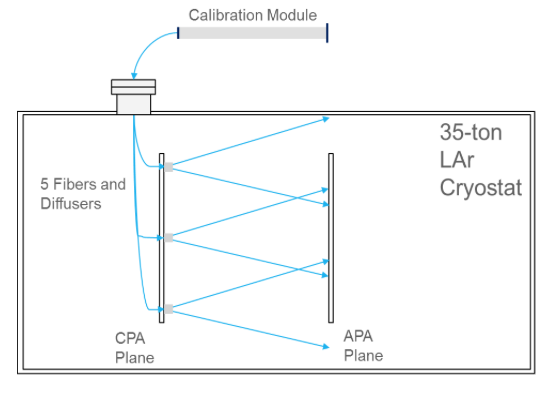
\includegraphics[width=.60\textwidth]{Figures/35tonpds.png}
%\includegraphics[width=.20\textwidth]{Figures/Diff1.png}
\end{dunefigure}

%There won’t be dedicated ports for all calibration devices. Therefore, multi-purpose ports are planned to be shared between various groups.
The calibration and the SP-PDS groups will define ports for optical feedthroughs. It is possible that SP-PDS might use \dword{dss} ports or TPC signal ports for routing fibers. The calibration group in coordination with other groups will provide a scheme for %interlock mechanism of operating various calibration devices 
an interlock mechanism to be used when operating various calibration devices (e.g., laser, radioactive sources) to avoid any damage to the \dwords{pd}. A dedicated firmware and software system will enable UV-light system to interface with DAQ and slow controls to communicate the start and stop of calibration runs, and issue commands to define types (amplitude, timing, frequency) of calibration pulses. Protocols will be defined with the DAQ group. 

 

\subsubsection{Remaining Studies}
The remaining studies %planned 
for the photon calibration system prior to the TDR include:
\begin{itemize}
\item Testing of components of the proposed \dword{pd} calibration system with \dword{protodune}. Additional tests will be launched between the SP photon detector and HV groups as needed, including a test stand with shared responsibility. 
\item %HV system will verify high voltage design and operation without discharges that could cause light emission observed by photon detector system should this be a concern. 
Verification that the HV system operates without discharges that could cause light emission observable by the \dword{pds}, should this be a concern.
\item Operate the proposed photon calibration system in \dword{protodune} %will be used to operate the  
and define the related DAQ needs for the \fardet.
%\item Determine if the PDS system may be used to emit electrons
\end{itemize}

